\documentclass[tikz]{standalone}
\usepackage{pgfplots}
\pgfplotsset{compat=1.15}
\usepackage{mathrsfs}
\usetikzlibrary{arrows,calc}
\usepackage{tkz-euclide}
\pagestyle{empty}

\definecolor{AngleClr}{rgb}{0,0.39215686274509803,0}
\definecolor{ShapeClr}{rgb}{0.6,0.2,0}
\definecolor{BlueClr}{RGB}{5,81,163}
\definecolor{RedClr}{RGB}{201, 20, 20}

\begin{document}

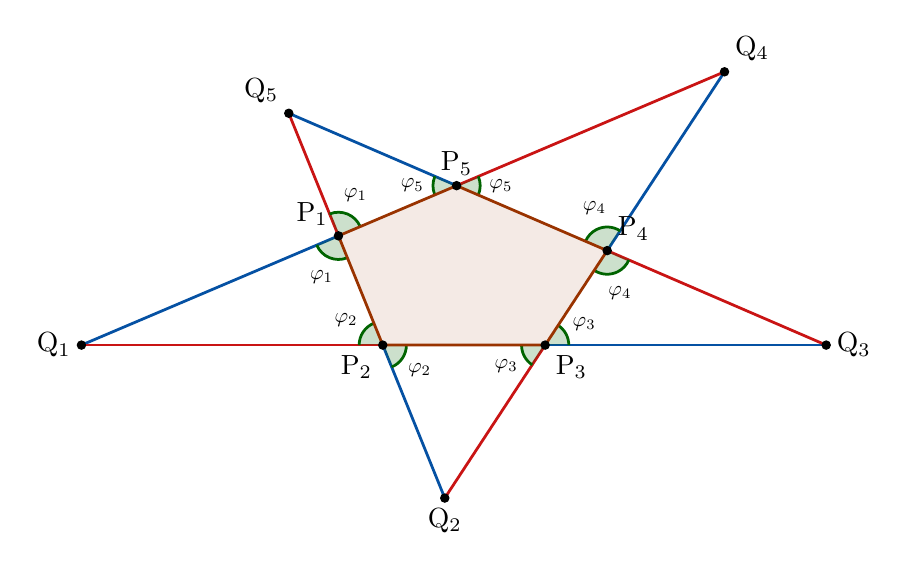
\begin{tikzpicture}[scale=.75]
\tkzSetUpLine[line width=1pt,color=black]
\tkzSetUpPoint[fill=black]

\tkzDefPoints{0/0/B,2.75/0/C,-0.75/1.85/A,1.25/2.7/E,3.8/1.6/D}

\tkzInterLL(A,B)(C,D) \tkzGetPoint{A1}
\tkzInterLL(B,C)(D,E) \tkzGetPoint{A2}
\tkzInterLL(C,D)(E,A) \tkzGetPoint{A3}
\tkzInterLL(D,E)(A,B) \tkzGetPoint{A4}
\tkzInterLL(E,A)(B,C) \tkzGetPoint{A5}

\tkzFillPolygon[fill=white](A,B,C,D,E)
\tkzFillPolygon[fill=ShapeClr,fill opacity=0.1](A,B,C,D,E)

\tkzDrawSegments[BlueClr](A1,B)
\tkzDrawSegments[BlueClr](A2,C)
\tkzDrawSegments[BlueClr](A3,D)
\tkzDrawSegments[BlueClr](A4,E)
\tkzDrawSegments[BlueClr](A5,A)

\tkzDrawSegments[RedClr](A1,C)
\tkzDrawSegments[RedClr](A2,D)
\tkzDrawSegments[RedClr](A3,E)
\tkzDrawSegments[RedClr](A4,A)
\tkzDrawSegments[RedClr](A5,B)


\tkzFillAngles[fill=AngleClr,size=.4,fill opacity=0.2](A5,A,B E,A,A4)
\tkzMarkAngles[line width=1pt,size=.4,color=AngleClr](A5,A,B E,A,A4)
\tkzLabelAngles[scale=0.75,pos=1](A5,A,B E,A,A4){$\varphi_1$}

\tkzFillAngles[fill=AngleClr,size=.4,fill opacity=0.2](A1,B,C A,B,A5)
\tkzMarkAngles[line width=1pt,size=.4,color=AngleClr](A1,B,C A,B,A5)
\tkzLabelAngles[scale=0.75,pos=1](A1,B,C A,B,A5){$\varphi_2$}

\tkzFillAngles[fill=AngleClr,size=.4,fill opacity=0.2](A2,C,D B,C,A1)
\tkzMarkAngles[line width=1pt,size=.4,color=AngleClr](A2,C,D B,C,A1)
\tkzLabelAngles[scale=0.75,pos=1](A2,C,D B,C,A1){$\varphi_3$}

\tkzFillAngles[fill=AngleClr,size=.4,fill opacity=0.2](A3,D,E C,D,A2)
\tkzMarkAngles[line width=1pt,size=.4,color=AngleClr](A3,D,E C,D,A2)
\tkzLabelAngles[scale=0.75,pos=1](A3,D,E C,D,A2){$\varphi_4$}

\tkzFillAngles[fill=AngleClr,size=.4,fill opacity=0.2](A4,E,A D,E,A3)
\tkzMarkAngles[line width=1pt,size=.4,color=AngleClr](A4,E,A D,E,A3)
\tkzLabelAngles[scale=0.75,pos=1](A4,E,A D,E,A3){$\varphi_5$}

\tkzDrawPolygon[color=ShapeClr](A,B,C,D,E)
\tkzDrawPoints[size=3](A,B,C,D,E)
\tkzDrawPoints[size=3](A1,A2,A3,A4,A5)


\tkzLabelPoint[above left](A){$\rm P_1$}
\tkzLabelPoint[below left](B){$\rm P_2$}
\tkzLabelPoint[below right](C){$\rm P_3$}
\tkzLabelPoint[above right](D){$\rm P_4$}
\tkzLabelPoint[above](E){$\rm P_5$}

\tkzLabelPoint[below](A1){$\rm Q_2$}
\tkzLabelPoint[right](A2){$\rm Q_3$}
\tkzLabelPoint[above right](A3){$\rm Q_4$}
\tkzLabelPoint[above left](A4){$\rm Q_5$}
\tkzLabelPoint[left](A5){$\rm Q_1$}

\end{tikzpicture}

\end{document}
